\chapter{Optimització i Ajustos}
\textbf{Mètodes d'Optimització en Intel·ligència Artificial:Fonaments i Aplicacions}\\
   \textbf{Introducció}\\
La Intel·ligència Artificial (IA) integra múltiples estratègies d'optimització, cadascuna adaptada als diferents models d'IA. A continuació, s'exploren els mètodes més destacats, amb un anàlisi dels mecanismes i les referències acadèmiques que hem utilitzat.

\begin{enumerate}
 \item \textbf{Retropropagació en Aprenentatge Profund:} La retropropagació (\textit{backpropagation}) és com el punt i coma en el text per les xarxes neuronals artificials. Aquest algorisme es basa en un procés iteratiu en dues fases:
    \begin{enumerate}
     \item \textbf{Fase de propagació endavant}: Les dades d'entrada es transmeten a través de les capes de la xarxa, generant una predicció. Durant aquest procés, cada neurona aplica una transformació lineal seguida d'una funció d'activació no lineal, com \textit{\hyperlink{subsec:1}{funció unitat rectificada uniforme}} o \textit{\hyperlink{3.7.1}{funció sigmoide}}.

     \item \textbf{Fase de propagació enrere}: Es calcula l'error entre la predicció i el valor real utilitzant una funció de pèrdua (\textit{loss function}), com l'error quadràtic mitjà (\textit{Mean Squared Error}) per a problemes de regressió o l'entropia creuada (\textit{Cross-Entropy Loss}) per a classificació. Mitjançant \nameref{subsec:cadena} (\textit{chain rule}), es determina la contribució de cada paràmetre a l'error global, obtenint els gradients $\partial L/\partial W$, on $L$ representa la pèrdua i $W$ els pesos de la xarxa.

     \item \textbf{Actualització de paràmetres}: Els pesos s'ajusten en la direcció oposada al gradient, utilitzant variants del descens de gradient, com SGD \textit{\nameref{subsec:gradient}}, que aplica updates amb un subconjunt aleatori de dades, o optimitzadors més sofisticats com Adam (\textit{Adaptive Moment Estimation}), que adapta la taxa d'aprenentatge per a cada paràmetre.
    \end{enumerate}
 Per més informació també podeu accedir aquest  aparatat \ref{subsec:propagació} on també explica la retropropagació de la xarxa neuronal.

 \textbf{Suport teòric}:
 \begin{quote}
 \textit{Rumelhart, D. E., Hinton, G. E., \& Williams, R. J. (1986). ``Learning representations by back-propagating errors.'' Nature, 323(6088), 533-536.}

 Aquest article seminal estableix els fonaments matemàtics de la retropropagació, demostrant la seva eficàcia per a l'entrenament de xarxes multicapa.
 \end{quote}

 \item \textbf{Optimització en Models Generatius:} Els models generatius, com les xarxes generatives adversàries (GANs) i els autoencoders variacionals (VAEs), empren tècniques d'optimització especialitzades.\\
 \textbf{Exemples:}\\

     \begin{enumerate}
      \item \textbf{Xarxes Generatives Adversàries (GANs):} El marc adversarial de les GANs implica la competició entre dos models:
          \begin{enumerate}
           \item \textbf{Generador (\textit{Generator})}: Transforma un vector de soroll/aleatori(\textit{noise vector}) en dades sintètiques, intentant enganyar el discriminador.

           \item \textbf{Discriminador (\textit{Discriminator})}: Distingeix entre dades reals i generades, actuant com un classificador binari.
          \end{enumerate}
           L'entrenament es formula com un joc minimax, on la funció objectiu és:
           $ \min_G \max_D V(D, G) = \mathbb{E}_{x \sim p_{\text{data}}}[\log D(x)] + \mathbb{E}_{z \sim p_z}[\log(1 - D(G(z)))] $

           La retropropagació s'aplica alternativament amb dues xarxes, ajustant els seus paràmetres per millorar les seves funcions respectives.

           \textbf{Suport teòric}:
           \begin{quote}
           \textit{Goodfellow, I., et al. (2014). ``Generative Adversarial Networks.'' Advances in Neural Information Processing Systems 27 (NeurIPS).}

           Aquesta publicació introdueix el concepte de GANs, destacant el seu potencial per a la generació de dades realistes mitjançant aprenentatge adversarial.
           \end{quote}

           \item \textbf{Autoencoders Variacionals (VAEs):} Els VAEs optimitzen l'\textit{Evidence Lower Bound} (ELBO), que combina dos termes:
               \begin{enumerate}
                \item \textbf{Terme de reconstrucció}: Minimitza l'error entre les dades originals i les reconstruïdes.

                \item \textbf{Terme de regularització}: Minimitza la divergència de Kullback-Leibler (\textit{KL divergence}) entre la distribució latent i una distribució prior (normalment una normal estàndard).

                L'optimització es realitza mitjançant gradient descent sobre l'ELBO, amb l'ajut del \textit{reparameterization trick} per a un càlcul eficient dels gradients.

                \textbf{Suport teòric}:
                \begin{quote}
                \textit{Kingma, D. P., \& Welling, M. (2013). ``Auto-Encoding Variational Bayes.'' arXiv preprint arXiv:1312.6114.}

                Els autors presenten el marc teòric dels VAEs, introduint tècniques clau com el \textit{reparameterization trick} per a l'entrenament eficient de models generatius probabilístics.
                \end{quote}
               \end{enumerate}
           \item \textbf{Aprenentatge per Reforç i Optimització basada en Polítiques:} En l'aprenentatge per reforç (\textit{Reinforcement Learning, RL}), l'optimització es centra en maximizar la recompensa acumulada. Un enfocament prominent és el \textit{Policy Gradient}, que ajusta directament la política (\textit{policy}) mitjançant:
           \[ \nabla_\theta J(\theta) = \mathbb{E}_{\tau \sim \pi_\theta} \left[ \sum_{t=0}^T \nabla_\theta \log \pi_\theta(a_t|s_t) \cdot R(\tau) \right] \]
           on $\tau$ representa una trajectòria i $R(\tau)$ la recompensa acumulada.
           \textbf{Suport teòric}:
           \begin{quote}
           \textit{Sutton, R. S., et al. (2000). ``Policy Gradient Methods for Reinforcement Learning with Function Approximation.'' Advances in Neural Information Processing Systems 12 (NeurIPS).}

           Aquest treball estableix les bases teòriques dels mètodes de gradient de polítiques, demostrant la seva aplicabilitat en entorns complexos.
           \end{quote}
           \textbf{Alternatives a la Retropropagació: Algorismes Evolutius:} Per a problemes on el càlcul de gradients no és factible, els algorismes genètics (\textit{Genetic Algorithms, GA}) ofereixen una solució viable. Aquests algorismes emulen l'evolució natural mitjançant:
               \begin{enumerate}
                \item \textbf{Selecció}: Els individus més aptes (\textit{fitness}) tenen major probabilitat de reproduir-se.

                \item \textbf{Creuament (\textit{Crossover})}: Combina característiques de dos individus per generar descendència.

                \item \textbf{Mutació}: Introdueix variabilitat genètica aleatòria.
               \end{enumerate}
    \end{enumerate}


\end{enumerate}


           \textbf{Suport teòric}:
           \begin{quote}
           \textit{Holland, J. H. (1975). ``Adaptation in Natural and Artificial Systems.'' University of Michigan Press.}

           Holland formalitza els algorismes genètics, inspirant-se en els mecanismes de selecció natural per a resoldre problemes d'optimització complexos.
           \end{quote}

 \label{Algoritme_gradient}\textbf{Algoritme Gredient descendent}\\
         L'algoritme de Gradient descendent és un algoritme imprescindible en l'entrenament de les xarxes neuronals, i de la intel·ligència artificial. Primer de tot hem d'entendre que és un gradient i una funció d'error.

         \textbf{Gradient: } En les xarxes neuronals, un gradient és un vector que indica la direcció en la que es mou i amb quina intensitat per que la funció d'error cambii més ràpid respecte als pesos de la xarxa neuronal. Per calcular el gradient, s'utilitza la derivada parcial de la funció de pèrdua respecte als pesos.

        \textbf{Funció d'error: } La funció d'error tracta de determinar el error entre el valor estimat i el valor real, amb la finalitat d'optimitzar els paràmetres de la xarxa neuronal.

         L' objectiu de l'algoritme gradiant descendent és minimitzar la funció d'error, o també l'error entre la predicció, es a dir, trobar la funció de pèrdua mínima, per aconseguir-ho s'ha de trobar el valor mínim de la funció. La funció de pèrdua mínima significa que els errors dels paràmetres (pesos i biaixos) de la xarxa han de ser molt aproximades al valor real, on s'ajusten aquest paràmetres ja que no són exactes.


        \begin{figure}[t]
         \centering
         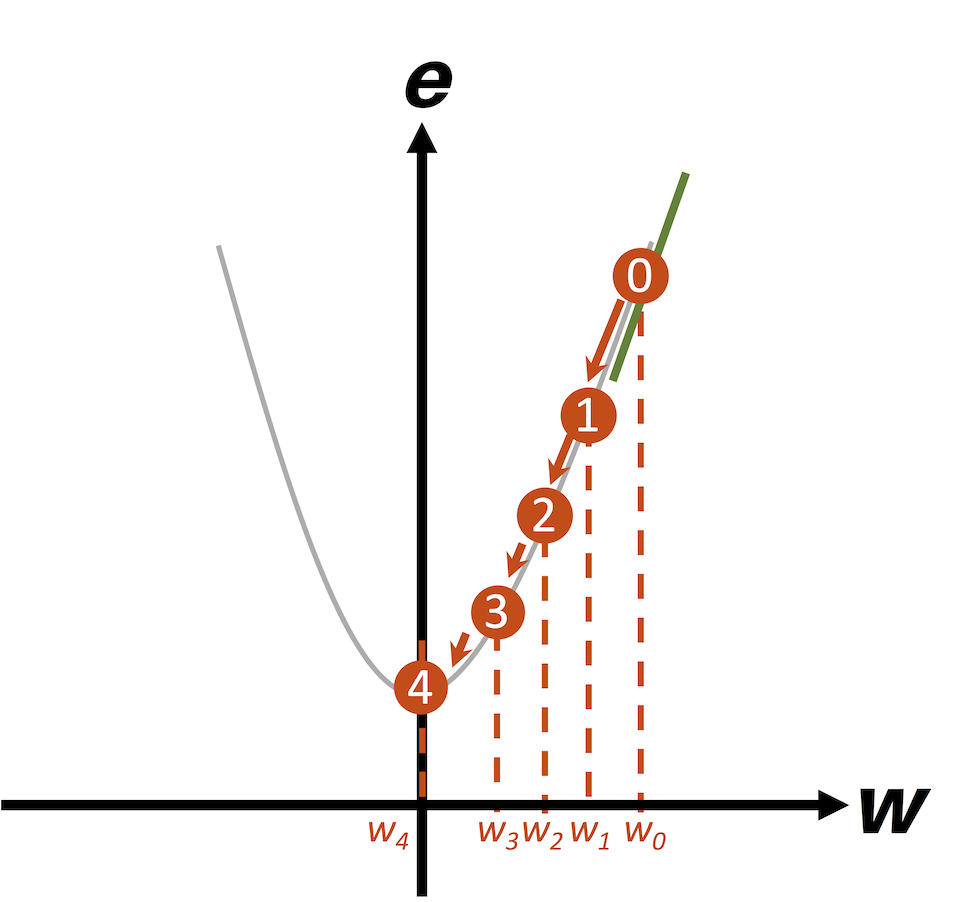
\includegraphics[width=0.5\textwidth]{./figures/gradient_descendent.png}
        \caption{Gràfica de gradient descendent}
        \label{GraficaDescendet}
         \end{figure}

          A la figura~\ref{GraficaDescendet}, on podem apreciar quatre iteracions, el valor inicial és un punt qualsevol de la funció. Al inici de la funció, en el punt 0, els paràmetres de la funció s'asignen aleatoriament, per tant els errors són grans. Desde aquell punt, trobarem la derivada parcial en cada una de les iteracions, i el gradiet serà l'encarregat de guiar els canvis als paràmetres.
          Al principi de tot, el gradient serà molt pronunciat, però a mesura que es van generant nous paràmetres durant l'entrenament, s'anirà reduint fins al put més baix d'aquesta corba, on els errors són molt petits, aquest punt se li diu punt de convergència. Aquí és on la xarxa ha après i ha ajustat millor les dades.

          La fòrmula del gradient ascendent és la seguent:
          $$\Delta w_{ij} = a \left( \frac{\partial E}{\partial w_{ij}} \right)$$
          Aquesta és la formula més ràpida per arribar al punt màxim dels gradients. Per tant la fòrmula del gradient descendent seria aquesta mateixa en negatiu, perquè és la forma més ràpida de trobar el punt mínim.
          $$\Delta w_{ij} = -a \left( \frac{\partial E}{\partial w_{ij}} \right)$$
          \textbf{Explicació de la fòrmula:}\\
           $\Delta w_{ij}$: Representa quant s'ajusta el pes en una iteració de l'entrenamen.

           $a$: És la constant d'aprenentatge, aquesta constant defineix quant afecta el gradiant en l'actualització dels nostres paràmetres en cada iteració. Si aquest valor és gran, cada iteració és molt gran, i el punt serà incapaç d'introduir-se al punt de convergència, causant que el procès d'optimització acabi en un bucle infinit. Tanmateix, si és petit, el punt s'aproxima poc a poc al punt de converència, però calcularà moltes iteracions i això pot ser ineficient.

           $\left( \frac{\partial E}{\partial w_{ij}} \right)$: És la derivada parcial de $E$ respecte a $\Delta w_{ij}$. \\

           A la figura~\ref{Gran i petit}, és una representació en 2 D, però en situacions reals el gradient descendent es representa en la dimensió 3 d.

\begin{minipage}[h]{0.45\textwidth}
    \begin{figure}[H]
    \centering
    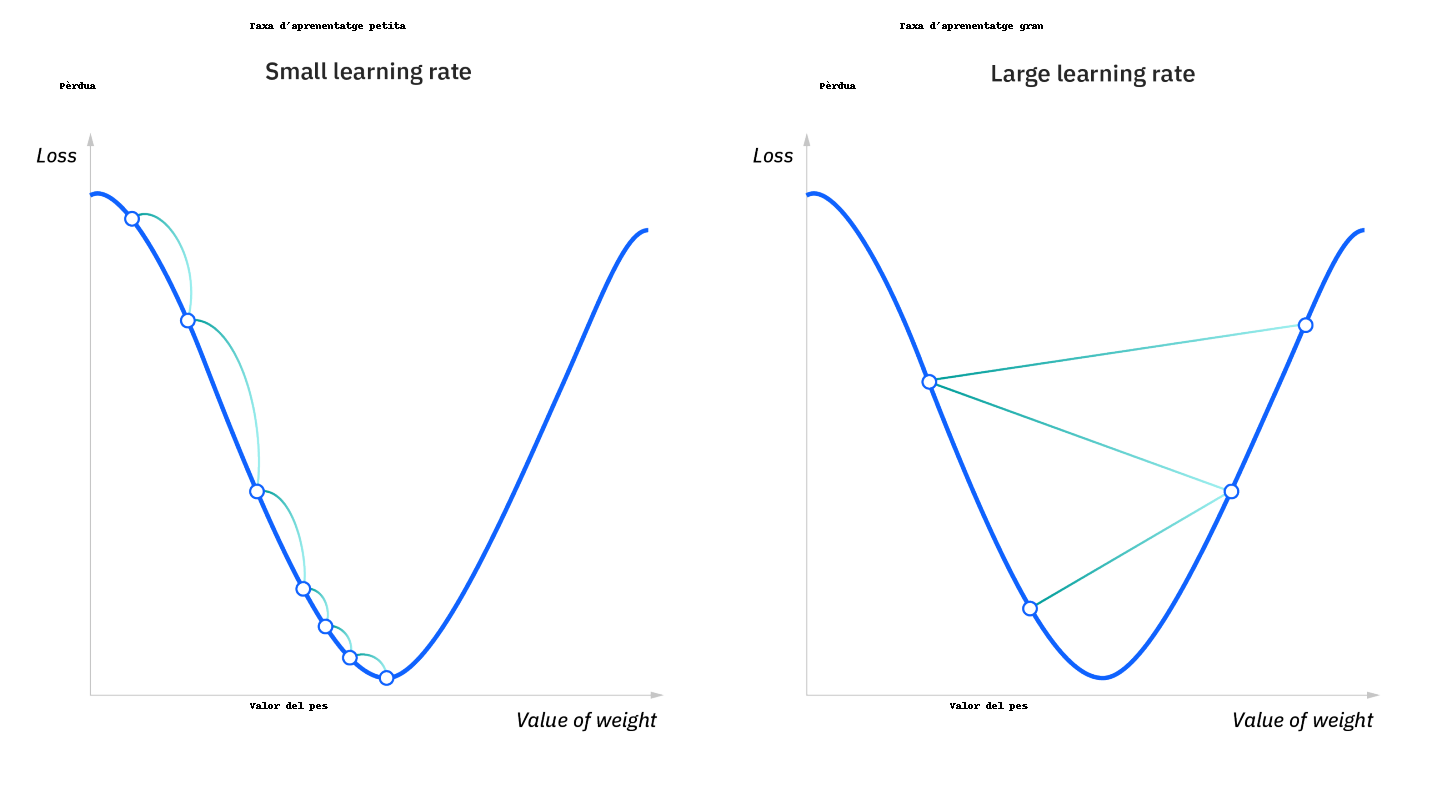
\includegraphics[width=1\textwidth]{./figures/constant_gradient.png}
        \caption{Gràfiques de valors gran i petit de la constant d'aprenentatge}
        \label{Gran i petit}
    \end{figure}
\end{minipage}
\begin{minipage}[h]{0.45\textwidth}
    \begin{figure}[H]
    \centering
    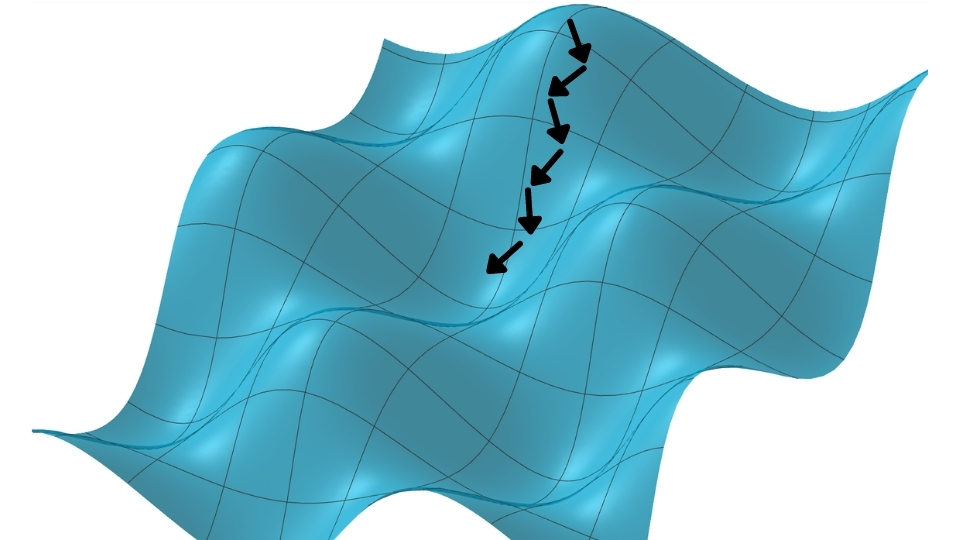
\includegraphics[width=1\textwidth]{./figures/gradient_descendent3d.png}
    \caption{Repressentació del gradient descendent en 3D}
    \end{figure}
\end{minipage}



            Fonts: ~\cite{IBM_Gradient} i ~\cite{Video_Gradient}.

 \textbf{Funció de pèrdua (o error)}\label{subsec:pèrdua}
     \hspace*{-1\leftmargin} Un sistema per avaluar l'encert de les prediccions, comparant-les amb resultats reals (quan es disposa d'ells). Si la predicció és incorrecta, aquesta funció quantifica la magnitud de l'error.
\subsection{La regla de la cadena}\label{subsec:cadena}

En l'aprenentatge automàtic, sovint es treballa amb funcions compostes complexes que depenen de diversos paràmetres i capes. Per tal de facilitar el càlcul dels gradients i optimitzar el rendiment computacional, s'utilitza la \textbf{regla de la cadena}.\\

La regla de la cadena és una tècnica de derivació matemàtica que permet descompondre la derivada d'una funció composta en el producte de derivades de les seves funcions internes. D’aquesta manera, es poden calcular les derivades de manera escalonada i eficient, especialment en el context de l’algorisme de propagació enrere (backpropagation).

Per exemple, si tenim una funció composta de la forma:

\[
L = f(g(h(x)))
\]

La derivada de \( L \) respecte a \( x \) s'obté aplicant la regla de la cadena:

\[
\frac{dL}{dx} = \frac{df}{dg} \cdot \frac{dg}{dh} \cdot \frac{dh}{dx}
\]

Aquest procediment és fonamental per entrenar xarxes neuronals, ja que permet calcular com cada pes de la xarxa contribueix a l'error global, i així ajustar-los mitjançant tècniques com el descens de gradient.

%fonts:\href{https://medium.com/%40ppuneeth73/the-chain-rule-of-calculus-the-backbone-of-deep-learning-backpropagation-9d35affc05e7}{Medium deep machine-learning} \ \href{https://www.geeksforgeeks.org/machine-learning/chain-rule-derivative-in-machine-learning/}{Greek machine-learning} Aquesta pàgina ja no existeix.
